\section{Qualitative Analysis}
\label{sec:qualitative}

\begin{figure}[h!]
    \centering
    \includegraphics[width=0.45\textwidth]{figures/AI_Project_Figure4_L1.drawio_cropped.pdf}
    \\[0.1cm] \textbf{Simple (L1)}
    \vspace{0.2cm}
    
    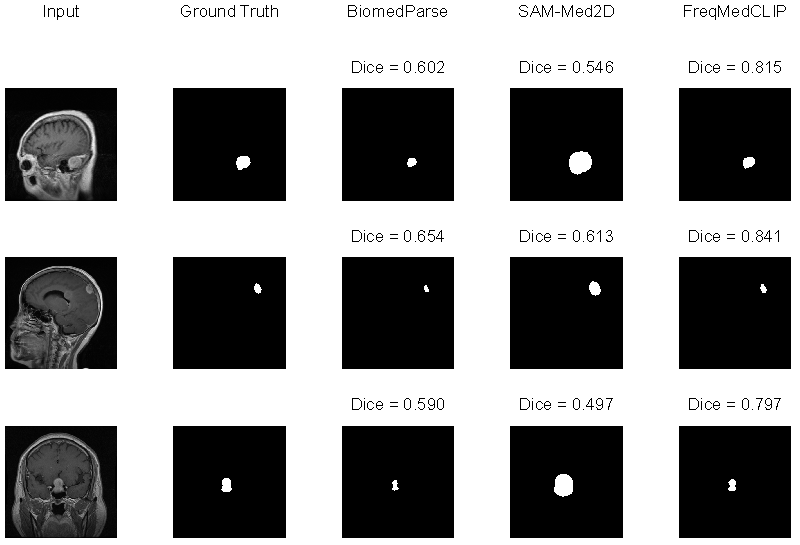
\includegraphics[width=0.45\textwidth]{figures/AI_Projects_Figure4_L3.drawio_cropped.pdf}
    \\[0.1cm] \textbf{Complex (L3)}

    \caption{\textbf{Qualitative Comparison.} The visual results confirm the quantitative metrics. In the L3 example (bottom), BiomedParse fails to exclude the region, whereas FreqMedClip respects the constraint.}
    \label{fig:qualitative_results}
\end{figure}

The qualitative examples in Fig.~\ref{fig:qualitative_results} illustrate the impact of the DPLG module. Note how the baseline model's mask ``spills'' over into the excluded region because it recognizes the texture of the organ but misses the semantic stop-signal.


In the ``Necrotic Core'' task, BiomedParse segments the \textit{entire} tumor, failing to distinguish the core. This confirms it treats the prompt as a generic class label (``Tumor''). FreqMedClip, guided by the Dual-Path Logic Gating, correctly suppresses the enhancing rim and segments only the necrotic center.

\FloatBarrier
